\chapter{Servizio Cittadino}

Il servizio cittadino (\emph{City Service}) è il cuore dell'architettura software e, al fine di supportare le interazioni tra gli EV e la Smart Grid. Lo scambio di informazioni avviene tramite un SIB cittadino e la struttura dei messaggi è definita all'interno dell'Ontologia. 

\section{Architettura}

Il principio di base con cui ho progettato il \emph{City Service} è la modularità e riusabilità. Ho quindi creato una libreria, \code{ioe_lib}, condivisa tra il servizio cittadino e l'applicazione mobile. Essa fornisce i servizi di base di accesso al \emph{SIB}, nonchè un approccio \emph{Object Oriented} ai dati in essa contenuti. Ho infatti implementato, per ogni classe presente nell'ontologia, una corrispettiva classe Entity Java e un \code{Controller} che incapsula la logica di lettura scrittura e aggiornamento dei dati nella \emph{SIB}. Questa scelta progettuale si rifà ai principi di Ingegneria del Software \emph{High Cohesion} e \emph{Low Coupling} \cite{larcab2005}

\section{La comunicazione con il City Service}\label{sec:protocol}

In questa sezione analizzeremo in dettaglio come avviene la comunicazione da e verso il servizio cittadino. Per ogni operazione esiste un protocollo basato su scambi di messaggi la quale struttura è definita attraverso classi dell'ontologia. Attualmente le uniche operazioni supportate sono la richiesta di prenotazione e la richiesta di ritiro di prenotazione.

Lo scambio dei messaggi è implementato tramite il meccanismo delle \code{Subscription} messo a disposizione dal SIB. Questo comporta che i messaggi vengono scritti sul \emph{SIB} cittadino il quale manda una notifica al \emph{KP} che era sottoscritto a quella particolare modifica. Questo rende il protocollo di comunicazione asincrono.


\subsection{Protocollo di richiesta di prenotazione}

Qui verranno descritti tutti i passaggi necessari al completamento del protocollo di Richiesta di Prenotazione, in particolare quali messaggi vengono scambiati. Il fine della Prenotazione è avere la certezza che quando andremo a caricarci troveremo l'EVSE libero. Come già detto in precedenza, i tempi di ricarica per i veicoli elettrici possono essere molto lunghi. È quindi necessario dare all'utente la sicurezza che potrà ricaricare il suo veicolo senza il rischio di terminare la batteria.

\begin{enumerate}[label=\textbf{\arabic*}]
	\item \textbf{Richiesta di Prenotazione}: Quando l'utente necessita di fare una ricarica inserisce una richiesta nel SIB. La richiesta è descritta dalla classe dell'ontologia \code{ioe:ChargeRequest}.
	\item \textbf{Risposta da parte del City Service}: Il servizio cittadino è sottoscritto all'inserimento di nuove istanze di \code{ioe:ChargeRequest}. Quindi, quando viene inserita la richiesta, arriva una notifica che ne contiene l'URI dal quale si possono ricavare tutti i parametri che la compongono. A questo punto viene creata una lista di opzioni di ricarica conformi alla richiesta dell'utente compatibilmente con la disponibilità degli EVSE. Le opzioni di ricarica sono classi di tipo \code{ioe:ChargeOption} e vengono inserite dentro a una classe di tipo \code{ioe:ChargeResponse}.
	\item \label{item:confirmByUser} \textbf{Conferma da parte dell'utente}: L'utente che è sottoscritto all'inserimento di nuove istanze della classe  \code{ioe:ChargeResponse} viene notificato quando il \emph{City Service} inserisce la risposta. Le opzioni di ricarica vengono analizzate dall'utente il quale sceglie quella che più si addice alle sue esigenze. La scelta viene notificata al sistema tramite inserimento di una tripla così formata: \code{[ioe:chargeOptURI ioe:confirmByUser "true"]} presupponendo che \code{ioe:chargeOptURI} sia un istanza di \code{ioe:ChargeOption}.
	\item \textbf{Conferma da parte del City Service)}: Il servizio cittadino è iscritto all'inserimento di triple che come predicato hanno \code{ioe:confirmByUser} e quindi verifica se l'opzione selezionata è ancora disponibile in tal caso inserisce una tripla siffatta:
	\\ \code{[ioe:chargeOptURI ioe:confirmBySystem "true"]}. 
	\item \textbf{Acknowledgment da parte dell'utente}: L'utente riceve la notifica della conferma da parte di \emph{City Service}. Se l'opzione è confermata allora invia una tripla di Acknowledgment \code{[ioe:userURI ioe:ackByUser "true"]}. Altrimenti può provare con un altra opzione e il protocollo riprende dal punto ~\ref{item:confirmByUser}
	\item \textbf{Creazione Prenotazione}: Quando il \emph{City Service} riceve l'acknowledgment dall'utente "blocca" l'EVSE nella finestra di tempo richiesta creando un istanza della classe {ioe:Reservation}. Inoltre cancella dal SIB tutte le triple necessarie allo svolgimento del protocollo che  , una volta terminato, diventano inutili.
\end{enumerate}

\section{Il Protocollo di rimozione di una prenotazione}

Una volta completata la procedura di prenotazione l'EVSE è diventa inagibile nell'orario richiesto dall'utente. Nel caso in cui un utente voglia ritirare la prenotazione deve mandare una richiesta al \emph{City Service}. Attualmente il servizio cittadino rimuove semplicemente dal SIB i dati relativi alla prenotazione rendendo nuovamente disponibile la ricarica. In futuro il servizio potrà stabilire, in base a regole dettate dai gestori della rete elettrica, se accettare o meno la richiesta ed eventualmente accreditare una penale all'utente.

Il Protocollo si basa su cambio di messaggi proprio come nel caso precedente.

\begin{enumerate}
	\item \textbf{Richiesta ritiro Prenotazione}: L'utente inserisce nel SIB cittadino un istanza della classe \code{ioe:ReservationRetire} 
	\item \textbf{Ritiro della Prenotazione}: Il \emph{City Service}, che ovviamente era sottoscritto alla creazione di nuove istanze di \code{ioe:ReservationRetire}, provvede a rimuovere dal SIB le triple relative alla Prenotazione.
	\item \textbf{Notifica avvenuta cancellazione}: Attualmente l'utente come unico modo per sapere dell'avvenuta cancellazione deve sottoscriversi ai cambiamenti dell'URI della Prenotazione che sta cancellando.
\end{enumerate}

\section{Implementazione}\label{sec:impl}

In questa sezione discuteremo i dettagli implementativi del \emph{City Service}, dalle tecnologie usate alle scelte Architetturali. Principalmente il serbizio cittadino deve essere altamente performante in quanto, una vota a regime, dovrebbe poter soddisfare le richieste di centinaia di utenti se non migliaia. Contemporaneamente bisogna preoccuparsi del fatto che l'alto parallelismo non intacchi l'integrità dei dati residenti sul SIB cittadino evitando, ad esempio, che due persone che fanno una prenotazione nello stesso momento, nello stesso EVSE, alla stessa ora non riescano entrambe a completare la procedura di prenotazione. 

Il servizio è scritto interamente in Java il che lo rende multi piattaforma, facile da debuggare, e sopratutto permette di usare utilità messe a disposizione del linguaggio per quanto riguarda il multithreading. Inoltre permette di accedere alla moltitudine di librerie scritte per questo linguaggio per i più disparati propositi. Tra queste troviamo (\code{log4j}), un robusto quanto versatile sistema di logging, che permette di tenere costantemente sotto controllo l'esecuzione del servizio con vari gradi di granularità del log.

Al fine di rendere il servizio più performante possibile sono state adottate tecniche di programmazione quali: pool di oggetti, pool di thread, e caching delle risorse.


\subsection{Pool Di Oggetti}

Per effettuare le connessioni al SIB cittadino è necessario istanziare oggetti di tipo \code{KpConnector}, inoltre, per effettuare il parsing delle risposte alle sottoscrizioni sono necessari oggetti di tipo \code{SSAP_XMLTools} che sono forniti dalla libreria \code{JavaKPI}. Come è stato detto nella sezione ~\ref{sec:impl} il \emph{City Service} deve supportare connessioni multiple simultanee, ognuna delle quali dialoga con il SIB. Dal momento che la libreria {JavaKPI} non è thread-safe e nemmeno il wrapper che ho creato io lo è, è necessario istanziare un oggetto \code{KpConnector} per ogni connessione insieme a uno di tipo \code{SSAP_XMLTools} per parsare i risultati delle sottoscrizioni.

Per evitare che all'avvio di ogni connessione venisse creato un oggetto \code{KpConnector}, che comunque è un oggetto "pesante", ho deciso di usare la tecnica dei pool di oggetti. La tecnica consiste nel creare un numero sufficienti di oggetti all'inizio dell'applicazione e quando si necessita di usarne uno lo si chiede al pool il quale lo fornisce al tempo di una chiamata a metodo. Una volta terminato di utilizzare l'oggetto lo si restituisce al pool il quale poi potrà a sua volta cederlo ad un altro richiedente.
In questo modo si evita che ogni volta che viene fatta una richiesta al \emph{City Service} ci sia il delay necessario a instanziare una connessione con il SIB.

C'è da dire che vista le ottimizzazioni delle moderne \emph{Java Virtual Machine} e del \emph{Garbage Collector} per quanto riguarda gli oggetti con breve durata questa tecnica può rischiare di abbassare le performance anziché aumentarle \cite{torok2011}. Rimane comunque vantaggiosa nel caso di oggetti la quale creazione può essere abbastanza onerosa come per le connessioni ai database o alla rete.

Il cuore di questo sistema è la classe \code{ObjectPool<T>} (\cite{objectpool}) che troviamo nel package \code{it.unibo.cityservice.pool} che rappresenta un pool di oggeti di tipo \code{T}. Questa classe contiene un metodo astratto \code{createObject()} che va implementato nelle sottoclassi mettendoci dentro la logica di creazione dell'oggetto di cui volgiamo creare il pool.

Nel mio caso ho creato \code{XmlToolsPool} e \code{CitySibPool} e a titolo esemplificativo mostrerò l'implementazione del primo:

\begin{java}[caption={Implementazione di ObjectPool},label={lst:objectPool}]
public class XmlToolsPool extends ObjectPool<SSAP_XMLTools>{
	
	public XmlToolsPool(final int minIdle) {
		super(minIdle);
	}

	@Override
	protected SSAP_XMLTools createObject() {
		return new SSAP_XMLTools();
	}
}
\end{java}

\noindent
Come si può vedere è molto semplice creare un pool per un determinato tipo di dato. Una volta creato il pool, per interagire con esso, si usano i seguenti metodi:

\begin{itemize}
	\item \code{public T borrowObject()}: che preleva un oggetto dal pool.
	\item \code{public void returnObject(T object)}: che restituisce un oggetto al pool.
\end{itemize}

\subsection{Pool Di Thread}

Adesso che abbiamo visto come è che cos'è il meccanismo dei pool degli oggetti e perchè è stato utilizzato vediamo invece di capire cosa sono i pool di thread e quali problematiche vanno a risolvere.
La creazione di thread può creare problemi in termini di performance (in quanto la creazione e distruzione di questo oggetti è abbastanza onerosa), di controllare il numero del numero dei thread creati e infine di scalabilità (\cite{vetti2008}).

Pertanto è necessario ricorrere alle classi del package \code{java.util.concurrent} che implementano l'interfaccia \code{Executor}. In questo caso sono state poi utilizzate istanze dell'interfaccia \code{ExecutorService} che mette a disposizioni metodi volti a controllare il ciclo di vita del pool stesso.

L'inizializzazione degli \code{ExecutorService} avviene tramite l'invocazione di un metodo statico della classe \code{Executors} che specifica la dimensione del pool che si vuole creare. Quando invece si vuole assegnare un compito ad uno dei thread del pool si usa il metodo \code{execute} che prende in ingresso un istanza dell'interfaccia \code{Runnable}.

\begin{java}[caption={Creazione Pool di Thread},label={lst:threadPool}]
ExecutorService pool = Executors.newFixedThreadPool(30);
pool.execute(new Runnable() {
	@Override
	public void run() {
		System.out.println("hello world");
	}
});
\end{java}

\subsection{Il funzionamento del City Service}
 
Come visto nella sezione ~\ref{sec:protocol} il servizio cittadino deve gestire un gran numero di messaggi a ogni tipologia dei quali corrisponde una sottoscrizione al SIB cittadino. Inoltre per poter rispondere alle richieste degli utenti deve anche avere le informazioni relative a tutti gli EVSE.

\subsubsection{Inizializzazione}\label{subsubsec:city-init}

Il \textsc{City Service} all'avvio compie innumerevoli compiti. Contrariamente a quanto avveniva in precedenza, dove i GCP erano codificati nell'ontologia e l'ontologia stessa veniva caricata da un programma esterno, ho deciso di delegare le inizializzazioni al \textsc{City Service} col fine di semplificarne lo sviluppo. Infatti in precedenza ad ogni riavvio del servizio era necessario uccidere manualmente il SIB e riavviarlo per avere una situazione di partenza pulita. Il caricamento dell'ontologia avviene tramite una libreria da me sviluppata, \emph{OntologyLoader}, (App. ~\ref{app:ontology-loader}) che a sua volta si appoggia alle librerie Apache Jena (\cite{jena2011}). In ambito di produzione ovviamente il servizio cittadino non eliminerebbe i dati e nemmeno ricaricherebbe quelli già presenti.

Di seguito una lista dettagliata delle operazioni eseguite dal \textsc{City Service} in fase di inizializzazione:

\begin{itemize}
	\item \textbf{Lettura file di configurazione}: Cerca il file di configurazione \code{cityservice.properties} dal quale carica le informazioni del SIB cittadino, il nome dell'ontologia, il nome del file contenente i GCP.
	\item \textbf{Scrittura Ontologia}: L'ontologia viene scritta nel SIB cittadino
	\item \textbf{Caricamento Informazioni GCP}: Le informazioni di tutte le stazioni di ricarica presenti in città vengono caricate da un file xml. Le stesse informazioni vengono inserite nel SIB al fine di poterle condividee con le altre entità del sistema.
	\item \textbf{Creazione Pool}: Vengono creati i pool di thred e di oggetti.
	\item \label{item:subscr} \textbf{Sottoscrizioni}: Ci si sottoscrive alle informazioni su cui si vuole rimanere aggiornate. Sostanzialmente ci si assicura che arrivino le notifiche per i messaggi descritti nella sezione ~\ref{sec:protocol}:
	\begin{enumerate}
		\item Creazione di nuove istanze di \code{ioe:ChargeRequest}
		\item Inserimento di triple contenenti come predicato \code{ioe:confirmByUser}
		\item Inserimento di triple contenenti come predicato \code{ioe:ackByUser}
		\item Creazione di nuove istanze di \code{ioe:ReservationRetire}
	\end{enumerate}
\end{itemize}

\subsubsection{Gestione delle richieste}

Quando ci si sottoscrive a qualcosa nel SIB oltre a definire a cosa ci vogliamo sottoscrivere dobbiamo anche definire un \emph{handler} che verrà eseguito quando avverrà il cambiamento a cui siamo interessati. Come visto sopra, nella sezione ~\ref{sec:protocol}, di sottoscrizioni ne vengono fatte 4, per ognuna di esse viene definito lo stesso \emph{hanlder} il quale lancia un thread istanza della classe \code{RequestDispatcher}. Esso si occupa semplicemente di gestire la richiesta e di eseguire un altro thread, sempre contenuto in un pool, che la soddisfi.

\paragraph{Sessioni}

Per ottenere un ulteriore incremento di performace è stato introdotto il concetto di sessione. La sessione inizia al quando il \emph{City Service} riceve la richiesta e finisce quando riceve l'acknowledgment. Il fine della sessione è mantenere una cache dei dati che vengono scambiati al fine di risparmiare query SPARQL, che sono assai onerose in termini di performance, e di dare un limite temporale alle sessioni stesse. La classe che si occupa di gestire le sessioni è \code{SessionManager} mentre la sessione è rappresentata dalla classe \code{session}.

All'interno della sessione vengono salvate le seguenti informazioni:

\begin{itemize}
	\item \textbf{chargeRequest}: Un istanza dell'entity \code{ChargeRequest} ricevuta all'utente. 
	\item \textbf{chargeResponse}: Un istanza dell'entity \code{ChargeResponse} inviata all'utente. 
	\item \textbf{reservation}: Un istanza dell'entity \code{Reservation} creata in seguito alla conferma dell'utente.
	\item \textbf{startTime}: Il momento in cui inizia la sessione.
	\item \textbf{endTime}: Il momento in cui finisce la sessione che corrisponde all'arrivo dell'acknowledgment dell'utente.
\end{itemize}

\noindent
La classe \code{SessionManager} possiede un timer che a tempo prefissato lancia un thread che controlla le sessioni attive. Se una delle sessioni è attiva da molto tempo senza essere stata chiusa allora significa che probabilmente c'è stato un problema e quindi vengono rimossi dal SIB tutti i dati relativi alla sessione compresa la prenotazione.

\paragraph{Prenotazioni}

La gestione delle prenotazioni, una volta che sono state create e confermate dall'utente, è delegata alla classe \code{ReservationManager}. A suo interno vengono salvate in una cache le istanze di \code{Reservation} create. Quando arriva una nuova richiesta di prenotazione la verifica della disponibilità viene fatta su questa cache anziché sul SIB. Questo sempre al fine di ridurre gli accessi al database e il successivo parsing delle risposte.
Siccome l'uso di questa classe è altamente parallelo, ovvero possono accedervi molti thread contemporaneamente, viene utilizzata una mappa thread-safe messa a disposizione da java \code{ConcurrentHashMap}. Inoltre le operazioni di verifica di disponibilità delle prenotazioni vengono sono atomiche a livello di EVSE grazie a un lock per ognuno di essi. 

\paragraph{Thread}\label{par:thread}

Ci sono cinque classi diverse che implementano l'interfaccia \code{Runnable} ognuna delle quali ha il compito di gestire un determinato aspetto dei protocolli di richiesta. Ovviamente c'è un pool di esecuzione per ognuna di esse.

\begin{itemize}
	\item \code{RequestDispatcher}: È il thread che si occupa di smistare le richieste agli altri esecutori, viene eseguito ogni volta che arriva una notifica da una sottoscrizione. La decisione avviene in base all'id della sottoscrizione che viene assegnato in fase di inizializzazione ed immagazzinato all'interno di variabili globali. Il codice di questo del corpo di questo thread è mostrato nel listato ~\ref{lst:requestDispatcher} dive si nota chiaramente l'utilizzo del pool di oggetti e dei pool di thread nonché del \code{logger}. Questo approccio viene usato anche per gli altri thread con l'aggiunta del reperimento dei \code{KpConnector} dal relativo pool.
	\item \code{ChargeRequestHandler}: Viene eseguito quando un utente inserisce un istanza istanza di \code{ioe:ChargeRequest} nel SIB. Dalla sottoscrizione ne ricava l'URI e con l'apposito controller \code{ChargeRequestController} la trasforma in un Entity java istanza della classe \code{ChargeRequest}. I passaggi che dalla richiesta elaborano una risposta sono i seguenti:
	\begin{enumerate}
		\item Controllo di coerenza sulla richiesta. Se la richiesta non è valida allora viene inviata una risposta vuota. Altrimenti si procede con il resto delle operazioni.
		\item Viene creata un istanza di \code{Session} gestita dalla classe \code{SessionManager}.
		\item Scelta dei \emph{GCP} che si trovano nell'area scelta dall'utente tramite la libreria \code{UniboGeoTools}.
		\item Vengono ciclati tutti gli \emph{EVSE} appartenenti ai \emph{GCP} selezionati.
		\item Per ogni \emph{EVSE} vengono ricavati gli slot di tempo compatibili con la fascia oraria e la quantità di carica richieste dall'utente.
		\item Viene generata la risposta istanza dell'Entity \code{ChargeResponse}. Al fine di minimizzare lo scambio di dati attraverso la rete sopratutto per non penalizzare i dispositivi mobili, le richieste vengono filtrate. Vengono inviate le opzioni di ricarica provenienti dai 5 \emph{GCP} più vicini e ne vengono scelte al massimo 2 per ogni \emph{EVSE}
		\item La risposta viene trasformata inserita nel SIB tramite la classe \\ \code{ChargeResponseController}.
	\end{enumerate}
	\item \code{ConfirmByUserHandler}: Questo thread viene invocato quando l'utente scaglie un opzione di ricarica e semplicemente controlla che sia ancora disponibile. In tal caso crea la prenotazione in modo che nessun altro possa usare la colonnina nell'orario richiesto. Da notare che l'istanza di \code{ChargeOption} viene presa dalla cache contenuta nella sessione anziché tramite query SPARQL e che l'istanza di \code{Reservation} viene salvata nel gestore di prenotazioni \code{ReservationManager}.
	\item \code{AckByUserHandler}: Viene invocato quando l'utente conferma l'opzione di ricarica. A questo punto il protocollo può considerarsi terminato e quindi vengono eliminate tutte le informazioni ad esso relative dal SIB e la sessione associata. L'unica informazione che rimane è un istanza di \code{ioe:Reservation} nel SIB.
	\item \code{RetireReservationHandler}: Si occupa semplicemente di eliminare le istanze di \code{ioe:Reservation} dal SIB e le corrispettive informazioni nella cache contenuta in \code{ReservationManager}.
\end{itemize}

\begin{java}[caption={Corpo di RequestDispatcher},label={lst:requestDispatcher}]
SSAP_XMLTools xmlTools = xmlToolsPool.borrowObject();
String subscriptionID = xmlTools.getSubscriptionID(subscribeResult);

if (chargeRequestSubId.equals(subscriptionID)) {
	chargeRequestExecutor.execute(new ChargeRequestHandler(subscribeResult));
} else if (confirmByUserSubId.equals(subscriptionID)) {
	confirmByUserExecutr.execute(new ConfirmByUserHandler(subscribeResult));
} else if (ackByUserSubId.equals(subscriptionID)) {
	ackByUserExecutor.execute(new AckByUserHandler(subscribeResult));
} else if (retireReservationSubId.equals(subscriptionID)) {
	retireReservationExecutor.execute(new RetireReservationHandler(subscribeResult));
} else {
	logger.error("Unexpected subscription id: " + subscriptionID);
}

xmlToolsPool.returnObject(xmlTools);
\end{java}	


\section{Testing}

Aspetto fondamentale che ha caratterizzato lo sviluppo del \emph{City Service} è stata l'integrazione con test di unità che ne hanno assicurato la continuità di funzionamento durante le fasi di modifica e sviluppo.

Il framework utilizzato per eseguire il testing è \code{junit4}, un ottima libreria Java che tramite il meccanismo delle annotazioni permette di scrivere ed eseguire i test i maniera semplice ed efficace.

I test sono stati determinanti non solo per assicurare la stabilità del codice ma anche per testare le performance del sistema, soprattutto del SIB. 

\subsection{Test Protocolli}

Per testare i protocolli ho implementato un thread che svolgesse tutte lo operazioni necessarie per completare una richiesta di prenotazione ed il ritiro della stessa. L'incapsulamento della logica del protocollo di richiesta all'interno di un thread permette di fatto l'esecuzione multipla di istanze di quest'ultimo simulando quindi l'interazione di molteplici utenti. La classe delegata a svolgere questo compito è \code{ioe:ChargeProtocolTest} nel packacge \code{it.unibo.ioe.cityservice.chargeprotocol} situato nella cartella di test. All'interno di questa classe si trova una inner-class, \code{ReservationProtocol} che implementa \code{Runnable} rendendo quindi possibile la sua esecuzione all'interno di un thread separato. 

Per simulare le attese dell'utente è stato usato il meccanismo dei lock. Ogni fase del protocollo ha un suo lock che viene acquisito subito dopo l'invio messaggio (List. ~\ref{lst:request-lock}) e viene rilasciato al momento dell'esecuzione l'handler associato alla sottoscrizione della risposta (List. ~\ref{lst:response-handler}).

\begin{java}[caption={Inserimento della \code{CargeRequest} e attesa della risposta},label={lst:request-lock}]
chargeRequestController.insertChargeRequest(request);
synchronized (chargeResponseLock) {
	try {
		chargeResponseLock.wait();
	} catch (InterruptedException ex) {
		logger.error(ex.getMessage(), ex);
	}
}
\end{java}

\begin{java}[caption={Handler associato al messaggio di risposta},label={lst:response-handler}]
String subscriptionID = xmlTools.getSubscriptionID(xml);
if (chargeResponseSubId.equals(subscriptionID)) {
		[...]
		chargeResponsesUri = subscriptionResult.get(0);
		synchronized (chargeResponseLock) {
			chargeResponseLock.notify();
		}
	}
}
\end{java}
\\
\noindent
L'opzione di ricarica viene scelta casualmente tra quelle fornite, nel caso in cui venisse confermata dal sistema il thread preleva la corrispondente istanza di \code{Reservation} creata e controlla che i parametri in essa contenuti siano coerenti con quelli dell'opzione scelta.\\
Tutti i dati scambiati dal protocollo vengono testati se uno di essi dovesse fallire causerebbe la terminazione del protocollo stesso. A tal proposito \code{junit} mette a disposizione una serie di funzioni che permettono di fare asserzioni di ogni tipo al fine di validare i dati. Queste funzioni iniziano con il prefisso \code{assert}, un esempio si può vedere nel listato ~\ref{lst:assert}.

\begin{java}[caption={Risposta ricavata a partire dall'uri, test del risultato},label={lst:assert}]
response = chargeResponseController.findChargeResponse(chargeResponsesUri);
assertNotNull(response);
assertEquals(request.getUri(), response.getChargeRequestUri());
\end{java}

\subsection{Valutazione Performance}

L'esecuzione di molteplici istanze del protocollo di richiesta è stato determinante al fine di testare le performance del sistema in quanto ha permesso di capire quante richieste contemporanee potessero essere servite e quali fossero i colli di bottiglia. È stato infatti scoperto che arrivati a un certo numero di connessioni simultanee il SIB allunga i tempi di risposta fino a far scattare il \code{socket-timeout} della libreria JavaKPI, in quanto, come indicato nella Sez. ~\ref{subsec:sib}, il SIB comunica con l'esterno tramite protocollo \emph{TCP/IP}. Questa scoperta ha portato a trovare un bug che affliggeva il SIB stesso, il quale, una volta interrotta brutalmente la connessione con il socket di JavaKPI, dava seri problemi di memory-leak come si può ben vedere in Fig. ~\ref{fig:sib-memory-leak}. L'immagine l'ho presa dal mio computer e l'ho inviata agli sviluppatori di Smart-M3-B per dimostrare il problema. Si nota chiaramente il momento precedente all'uccisione del SIB in cui erano allocati circa 8GB di Ram e 3Gb di Swap. Il problema è stato risolto e la versione attuale (0.901) ne è esente.

\begin{figure}[H]
	\centering
	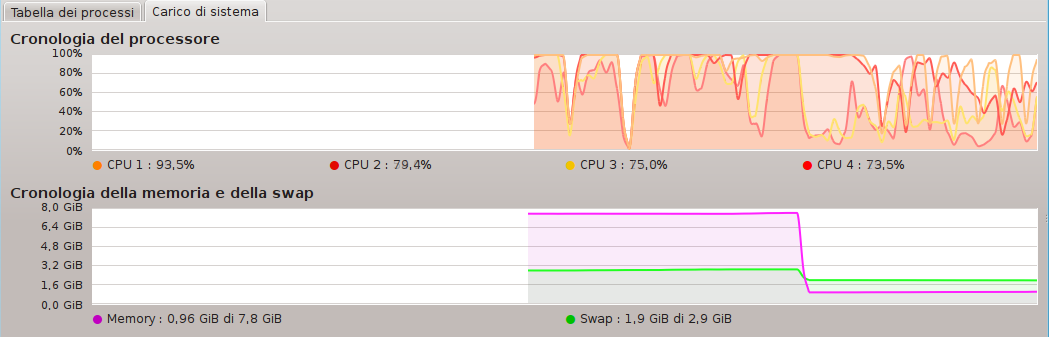
\includegraphics[width=1.0\textwidth]{assets/sib-memory-leak.png}
	\caption{Memory Leak del SIB che avveniva quando la connessione viene interrotta da un socket-timeout}
	\label{fig:sib-memory-leak}
\end{figure}

\noindent
La scoperta di questo problema ha portato quindi alla necessità di ottimizzare le performance, è stato quindi deciso di limitare il numero di risposte fornite dal servizio cittadino (Par. ~\ref{par:thread}) che causa un ingente traffico di dati da e verso il SIB. Altra ottimizzazione che decisa in seguito a queste scoperte è stata quella di trasformare le operazioni di INSERT di triple in query SPARQL, in quanto, grazie all'uso dei prefissi al posto degli URL interi, si riesce ad ottimizzare notevolmente il volume di dati scambiato, il che porta a notevoli vantaggi durante l'uso nell'applicazione mobile.









